\documentclass[conference]{IEEEtran}

\usepackage{hyperref}
\usepackage{graphicx}\graphicspath{ {images/} }
\usepackage{listings}
\usepackage{flushend}
\usepackage{caption}
\usepackage{xcolor}
\usepackage{lipsum}

% Hyphenation correction
\hyphenation{op-tical net-works semi-conduc-tor}


\begin{document}

\title{An Accessible, Open-Source, Realtime AODV Simulation in MATLAB}
\author{\IEEEauthorblockN{Stuart Miller}
\IEEEauthorblockA{Department of Electrical and\\Computer Engineering\\
Missouri University of Science \& Technology\\
Rolla, Missouri 65409\\
Email: \href{sm67c@mst.edu}{mailto:sm67c@mst.edu}\\
Web: \url{http://web.mst.edu/\textasciitilde sm67c}}
}

\maketitle

\begin{flushright}\end{flushright}
\begin{abstract}
It is often necessary to provide a base-level teaching tool when explaining concepts to new learners, or for the engineer performing initial basic prototyping. Understanding routing schemes in wireless ad-hoc networks is a central concept for any new learner. Since the subject is best taught through hands-on experience, many learners find themselves at a disadvantage when exposed to even more confusing and highly specialized tools used in wireless network simulation. Therefore, it is proposed to use the familiar and accessible environment of MATLAB to create base-level accessible, open-source, realtime ad-hoc routing scheme simulations, here targeting the ad-hoc on-demand distance vector  (AODV) routing scheme.
\end{abstract}

\section{Introduction}
One of the key advantages to using MATLAB as an environment is its natural support for high quality GUI displays. The suer interface is easy to understand and can be updated with simulation data in real-time. A major drawback to many preeminent network simulation tools is their reliance on written scripts and their inability to allow real time analysis and modification. MATLAB allows real-time input/output interaction and visualization. Additionally, it provides a much better debugging environment.

Perhaps most importantly, this work can provide a much more accessible intro to wireless routing schemes, as most engineers are already familiar with MATLAB functionality. Most network simulation scripting environments provide a significant barrier to enter due the their learning curve and often extensive environment setup time. MATLAB requires no setup beyond installation of the base program and is easy to understand. It follows that Stack Overflow listed MATLAB as one the least disliked languages of 2017 \cite{stack_overflow_disliked} and that 4.3\% of all contributors used MATLAB as their primary language \cite{stack_overflow_popularity} (although undoubtedly more are familiar with it causally).

For the purposes of this initial work, the focus will be on the ad-hoc on-demand distance vector  (AODV) routing scheme; however it is easy to see how the concepts here can be extended to additional routing methods.

\section{Literature Survey}

Although AODV was developed almost 15 years ago \cite{rfc3561}, it still remains highly studied in the current state of the art. The recent body of work shows much interest on the subject of AODV as a routing protocol. Several recent comparative analyses of routing protocols in MANET or VANET networks feature AODV: Ferrnato, et. al. in their protocol analysis with regards to urban vehicular scenarios \cite{aodv_interest_urban}, Abuashour and Kadoch in their study of clustered VANET scenarios \cite{aodv_interest_vanet}, and Ejmaa, et. al. in their modification of AODV to create a routing scheme with less RREQ message overhead \cite{aodv_interest_overhead}. The abundance of work in this area serves as assurance that AODV still remains a central protocol to the field and will serve as a relevant target protocol for this project.

While MATLAB does already provide a comprehensive WLAN systems toolbox \cite{matlab_wlan_toolbox}, it is solely targeted at IEEE 802.11 standards-compliant LAN-based networks and provides little-to-no support for ad-hoc or sensor networks. The selection of specified ad-hoc routing schemes and modification of node parameters is not present in the toolset provided. Unfortunately, this is far from sufficient for the goals of this endeavor.

The existing body of work does, however, show several instances of using MATLAB to test out highly specialized ad-hoc routing schemes. Gaur, et. al. show a novel routing scheme for optimizing battery life of the mica2 motes using MATLAB as a simluation environment \cite{matlab_ex_mica2}. Navya and Deepalakshmi utiltize MATLAB so show the feasibility of their proposed M-TSIMPLE routing protocal, an energy-efficient routing scheme for wireless body area networks \cite{matlab_ex_mtsimple}.  While both of these approaches do prove the feasibility of MATLAB as a simulation environment, each is far too specialized for the generalized application needed here.

Habib, et. al. describe another approach to the usage of MATLAB in this area: to simulate path-finding algorithms in various routing schemes, and to provide a comparison among networks of varied size \cite{matlab_ex_pathfinding}. Their analysis focuses more on the mathematics of pathfinding and as such, is also insufficient for our purposes.

While there is significant work being produced using MATLAB as an environment, much of the groudbreaking work is being done in other simulation tools as well. Network Simulator 3 (ns-3) a popular tool for such simulations; it provides a discrete-event network simluator/emulator and scripting language based on C++ or Python code \cite{ns3}. Ns-3 is targeted primarily for research and educational use. While popular, is has received significant criticism. Patel and Kmaboj criticized ns-3 harshly for it's lack of a GUI and noted it's complexity and lack of hosted work and support \cite{ns3_criticism}. That is not to say it is not without significant work in the academic community. Mai, et. al. used ns-3 to simulate their version of AODV, modified for a better congestion control scheme \cite{aodv_in_ns3}.

Another noteworthy platform is NetSim \cite{netsim}. Netsim Academic is the tool that most closely mirrors the intentions of this project as it is targeted at teaching/learning applications and provides adundant examples and support. Unfortunately, it is neither free nor open-source and requires a large license purchase to use. It is not without usage in the academic community though; numerous papers have cited NetSim as their primary simulation environment. Saifuddin, et. al. utilized NetSim in their analysis of alternative channel allocations for wireless networks \cite{netsim_spectrum}.  Nayak and Sinha provided an analysis of various mobility models for routing protocols (including AODV) using NetSim \cite{netsim_mobility}. Figure \ref{fig:netsim_example} shows an excerpt from their paper featuring their AODV simulation. A setup similar to the is the target for this MATAB implementation.

\begin{figure}[ht]
	\centering
 	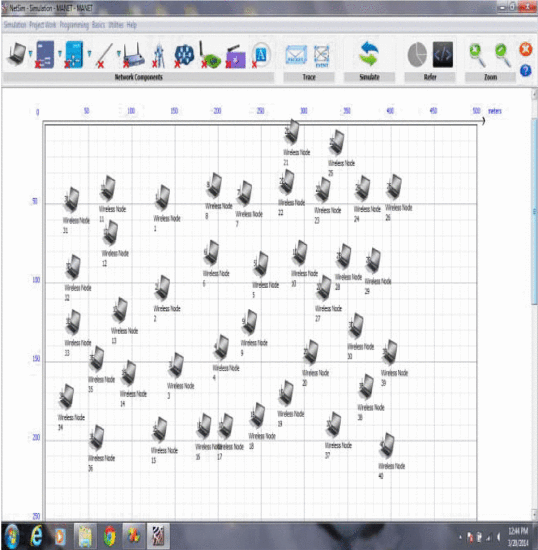
\includegraphics[width=2.79in]{netsim_example.png}
	\caption{Nayak and Sinha's AODV simulation window \cite{netsim_mobility}}
	\label{fig:netsim_example}
\end{figure}

Finally, OMNeT++ is yet another discrete-event library used frequency used to build network simulators \cite{omnet}. OMNeT sees quite a bit of use in the academic comnmunity as well, Chadha, et. al. used it in their simulation of energy consumption of nodes in a 3D environment \cite{omnet_efficient}.Thomas and Irvine investigate bandwidth usage in LTE sensor networks using OMNeT as a simulation tool \cite{omnet_lte}. Unfortunately, OmNeT falls into the same category as ns-3 in that it is overly complex and features far too steep of a learning curve to serve as a useful comparison for the objectives here.

\section{Methodology}

All of these simulation tools fall short in that they require a large learning curve; an engineering student or learner wishing to construct a prototype in any of these environments must first spend significant time learning the intricacies and methods of each. Furthermore, none are realtime and most provide little or no real support for visualization. MATLAB as an environment provides these features out of the box. Uluisik and Sevgi summarize this sentiment quite appropriately in their paper developing a MATLAB GUI for mapping complex functions\cite{matlab_gui}; after summarizing the existing body of work, they determined that an inherently simple and easy-to-operate MATLAB package was the best means to demonstrate the concepts they wished to teach. 

MATLAB provides a single high fidelity environment that facilitates both easy plotting of data and quickly creating robust user interfaces. The AODV simulation utilizes multiple figure windows that can simultaneously display different aspects of the algorithm's progress. It will also have the capability to plot statistical data afterwards.

The AODV simulation will start by allowing a layout scheme to be chosen and a set number of nodes to be plotted on a position grid (this project will focus on only 2-dimensional positional layouts). The user can add, remove, and manipulate nodes as desired and to create unique contrived network scenarios to test edge cases Each node will then be able to "flood" its nearest neighbors and build a local routing table. The user can then request packets be sent between two nodes and observe the path in real time.

As the intent of the project is to provide a basic level teaching and learning tool; the simulation in its current state will skip some aspect of wireless network simulation. Notably, this simulation does not implement queuing. Interference, sources of time delay, and power utilization are all removed so that the learner can focus more on the basic principles at play.

\section{Results}

\subsection{Example 1}

\begin{figure*}[ht]
	\centering
	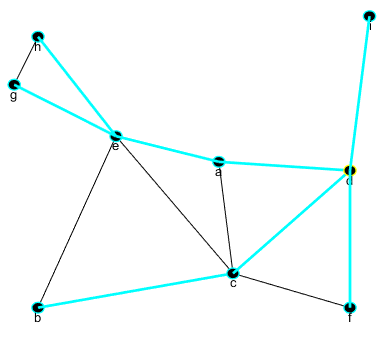
\includegraphics[width=2.1in]{Ex_1_request.png}
	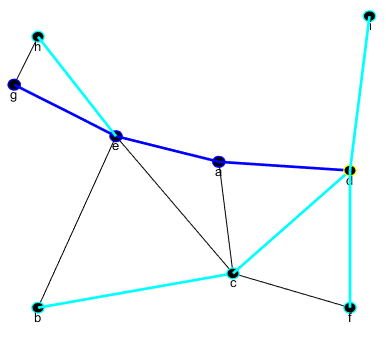
\includegraphics[width=2.1in]{Ex_1_reply.png}
	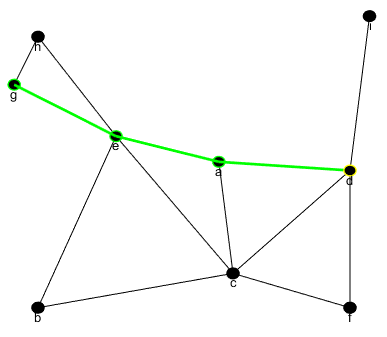
\includegraphics[width=2.1in]{Ex_1_data.png}
	\caption{Simple route request and reply, route messages \\
			\textcolor{cyan}{RREQ}, \textcolor{blue}{RREPL}, and \textcolor{green}{data} }
	\label{fig:ex_1}
\end{figure*}

\begin{figure*}[ht]
	\centering
	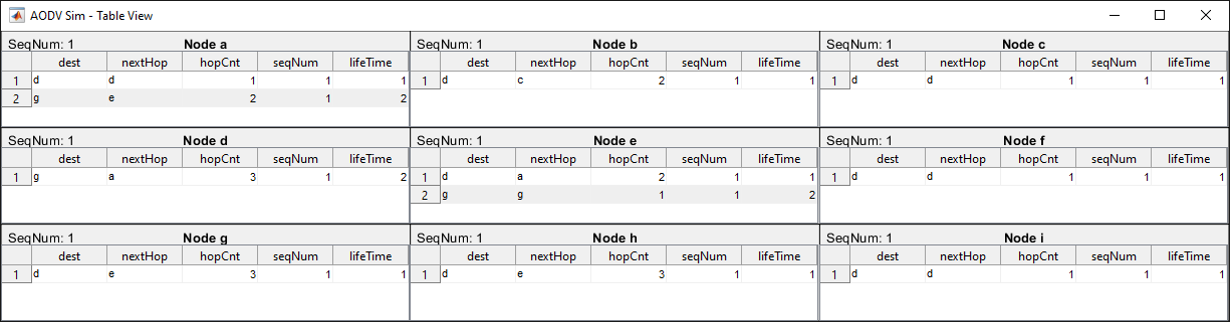
\includegraphics[width=6.8in]{Ex_1_table.png}
	\caption{Simple route request and reply, node route tables}
	\label{fig:ex_1_table}
\end{figure*}

The simplest scenario involves a node sending a transmission across the network with no prior knowledge whatsoever. Take the node layout in in figure \ref{fig:ex_1}. Lines show the available links to each node's nearest neighbors. A packet will be sent from node D to node G. D has no route to G so it emits a route request (RREQ), which is forwarded by each node that receives it and thus propagates throughout the network via "flooding" (notated by the cyan links). Along the way, each node sets up reverse route entries detailing the next node, hop count, and sequence number in order to send to the source of the route request. Upon receiving the request, node G replies with a route reply (RREPL)(notated by the blue links), which the intermediate nodes know how to direct thanks to the reverse routes that were just set up. Finally, now that D has a valid route to G, data is sent (notated by the green links). Subsequent transmissions to G from D will continue to use this route and require no new overhead.

As an aside, this simulation does not visualize any RREQ messages that are not acknowledged. In reality, each node is sending out RREQs in all directions, including the direction that it just received it's own RREQ from, but that node will discard it upon receipt.

Upon completion, each node's route table can be ovserved in the figure \ref{fig:ex_1_table}. Note that nodes contain a reverse route entry for D thanks to the flooding. Nodes  A, D, and E are along the data path and contain routes to G.

\subsection{Example 2}

\begin{figure*}[ht]
	\centering
	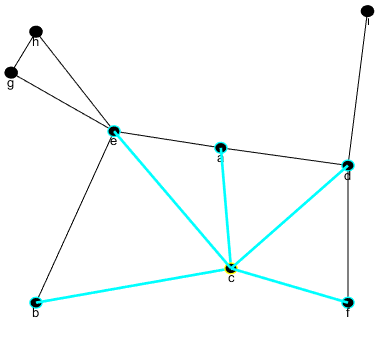
\includegraphics[width=2.1in]{Ex_2_request.png}
	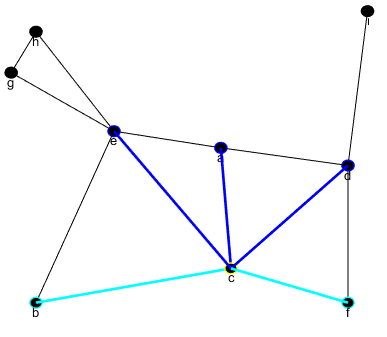
\includegraphics[width=2.1in]{Ex_2_reply.png}
	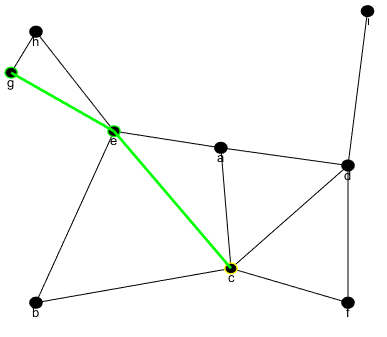
\includegraphics[width=2.1in]{Ex_2_data.png}
	\caption{Route request and reply from intermediate nodes, route messages \\
			\textcolor{cyan}{RREQ}, \textcolor{blue}{RREPL}, and \textcolor{green}{data} }
	\label{fig:ex_2}
\end{figure*}

\begin{figure*}[ht]
	\centering
	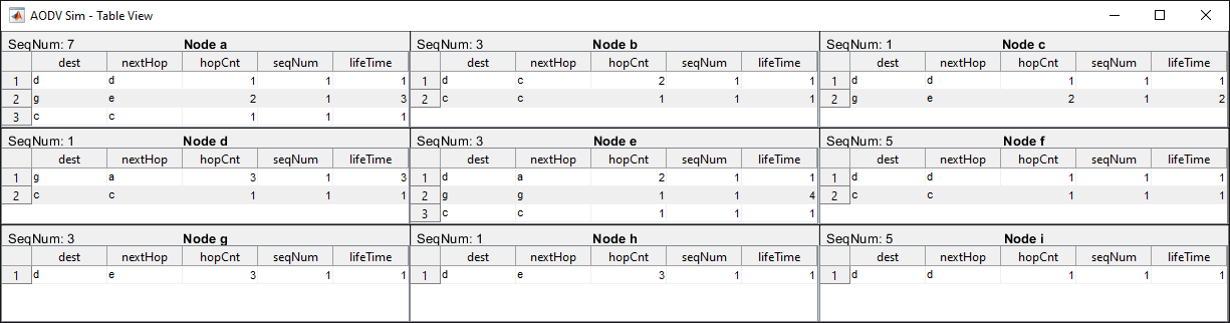
\includegraphics[width=6.8in]{Ex_2_table.png}
	\caption{Route request and reply from intermediate nodes, node route tables}
	\label{fig:ex_2_table}
\end{figure*}

Example 2 involves utilized the previously stored route tables (figure \ref{fig:ex_2}. In this case, node C will try sending to node G. Since C contains no entry for G in its route table, it must flood; however, the intermediate nodes A, D, and E all do have entries for G. Instead of propagating the RREQ message onward, they respond with a RREPL. C updates its route table upon receipt of each RREPL, choosing the route with the lowest hop count to G each time. Eventually, C is able to send out to E, who the continues to send to G via its route entry established in Example 1.

Again, the route table is shown in figure \ref{fig:ex_2_table}. Note the additional entries in A, B, D, E, and F.

\subsection{Example 3}

\begin{figure*}[ht]
	\centering
	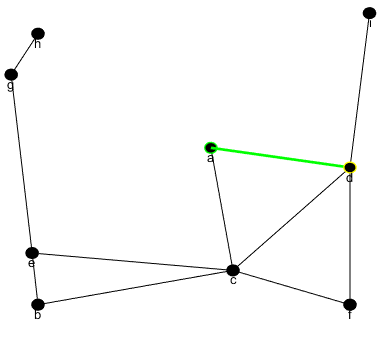
\includegraphics[width=2.1in]{Ex_3_data_1.png}
	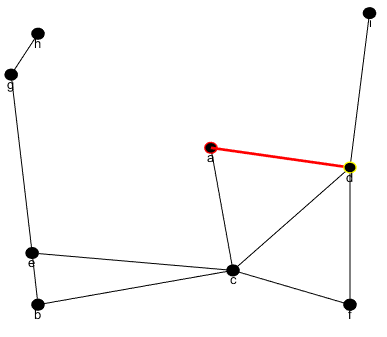
\includegraphics[width=2.1in]{Ex_3_error.png}
	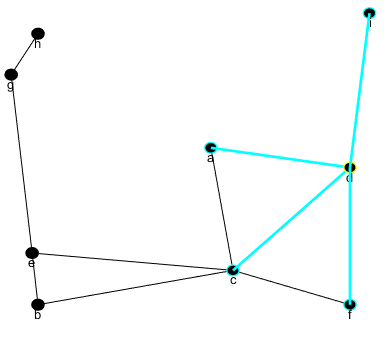
\includegraphics[width=2.1in]{Ex_3_request.png}
	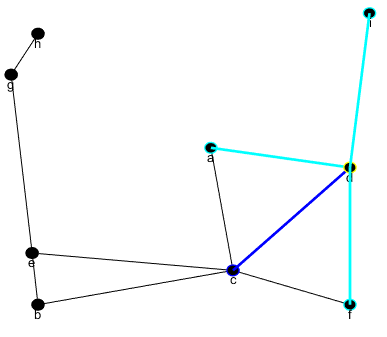
\includegraphics[width=2.1in]{Ex_3_reply.png}
	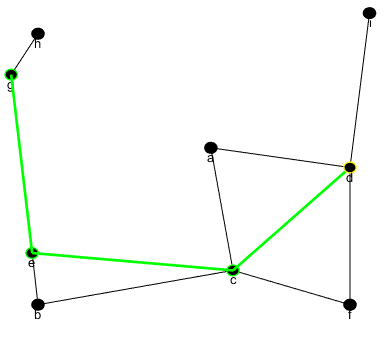
\includegraphics[width=2.1in]{Ex_3_data_2.png}
	\caption{Link breakage, route messages \\
			\textcolor{cyan}{RREQ}, \textcolor{blue}{RREPL}, and \textcolor{green}{data} }
	\label{fig:ex_3}
\end{figure*}

\begin{figure*}[ht]
	\centering
	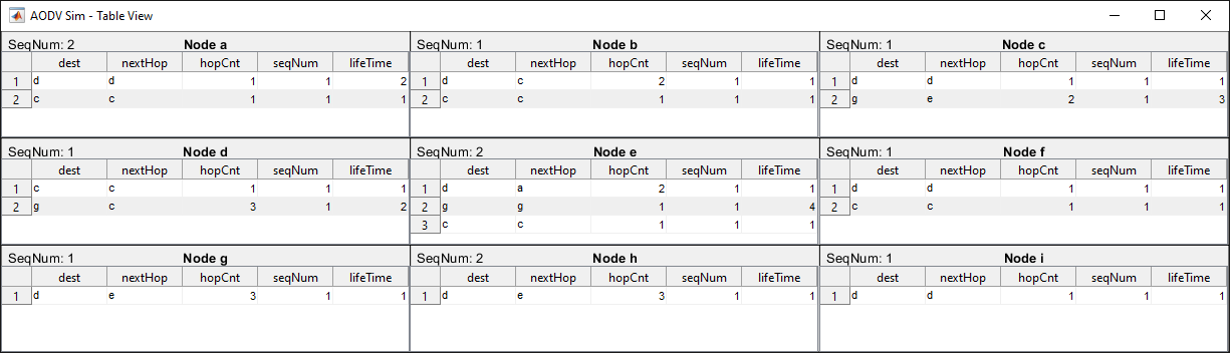
\includegraphics[width=6.8in]{Ex_3_table.png}
	\caption{Link breakage, node route tables}
	\label{fig:ex_3_table}
\end{figure*}

One of the most beneficial features of AODV is its elegant handling of link failures. A link failure occurs when a pre-established route is no longer possible due to node movement or interference. AODV handles this by sending route error (RERR) messages, as shown in figure \ref{fig:ex_3}. In this example, node D once again tries to send to node G, but intermediate node E has moved, breaking the route. D starts off by trying to send normally, but A must reply with a RERR when it realizes it can't reach E. This message propagates back up to D and both nodes cancel out their routes to G. D must once again flood by sending out RREQ packets. C replies that it knows a route (the one established in example 2) and D then proceeds to send to G via C.

The subsequent routing table is shown in figure \ref{fig:ex_3_table}. The sequence number have increased several times. Each time the nodes notice a change in their local network topology the increase their sequence numbers. All nodes connected or disconnected from E have been incremented to 2.

While this is an exceptional method of handling single link failure or small changes in topology, it starts to become rather burdensome when multiple route failures occur. One can imagine a contrived highly mobile scenario where the topology changes in such a way as to allow every intermediate node to obtain a false route entry for the desired destination. In such a case, the source node must attempt to send and receive a reply. It then floods but receives multiple replies. Because AODV provides no method of maintaining a node's past activity, it must attempt sending again, receive an error, flood again, attempt to send again, etc. It can only cancel out one intermediate node's route destination entry at a time, potentially causing enormous overhead.

\section{Analysis}

To investigate the problem of quantifying exactly how much overhead various network topologies generate, statistics from several repeated transmissions were aggregated. In each simulation, the network had it's nodes reset to an established starting position and the route tables for all nodes were cleared. Nodes were set in motion and updated their position regularly. Each node had a pre-established step size and direction. Nodes reflected off the boundaries of the simulation area in order to ensure that they stayed relatively close to each other and did not go out of bounds. Random traffic was generated and sent through the network. The random number generator used a static seed to ensure that all variables were consistent from experiment to experiment. 

\begin{figure}[ht]
	\centering
	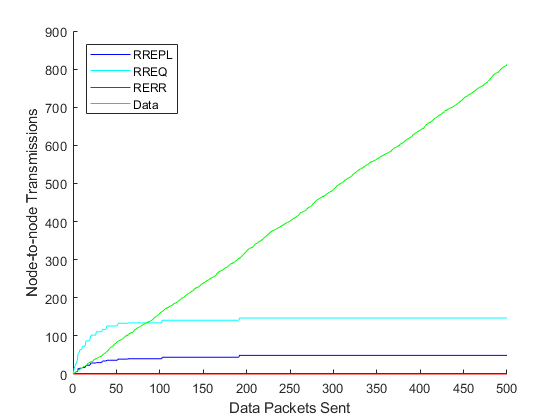
\includegraphics[width=3in]{movement_none.png}
	\caption{Network overhead with static nodes}
	\label{fig:movement_none}
\end{figure}

To begin with, traffic was evaluated on a static network (figure \ref{fig:movement_none}).
Here, the number of RREQ messages steadily increases until around the 50th packet, at which time most nodes have all possibly connections mapped out. The data rate climbs steadily since no transmissions fail and the RERR rate is accordingly zero.

A more realistic scenario may involve more frequent movement. Figure \ref{fig:movement_50} shows overhead with movement every 50 packets and figure \ref{fig:movement_10} with movement every 10 packets. The frequent movement in figure \ref{fig:movement_10} finally surpasses the data rate and would likely be enough to overwhelm the controllers on most realistic nodes. In such a high mobility case, a specialized routing algorithm would likely need to be utilized as AODV's performance is lacking here.

\begin{figure}[ht]
	\centering
	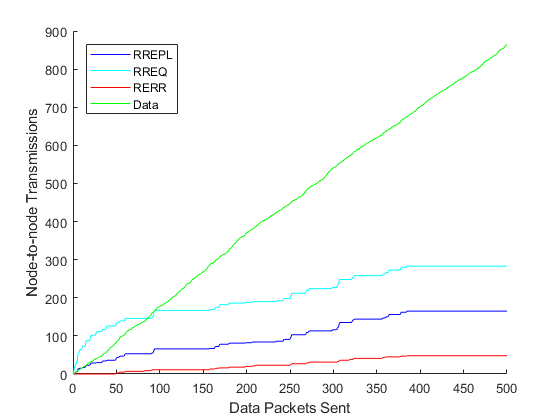
\includegraphics[width=3in]{movement_50.png}
	\caption{Network overhead with nodes moving every 50 packets sent}
	\label{fig:movement_50}
\end{figure}

\begin{figure}[ht]
	\centering
	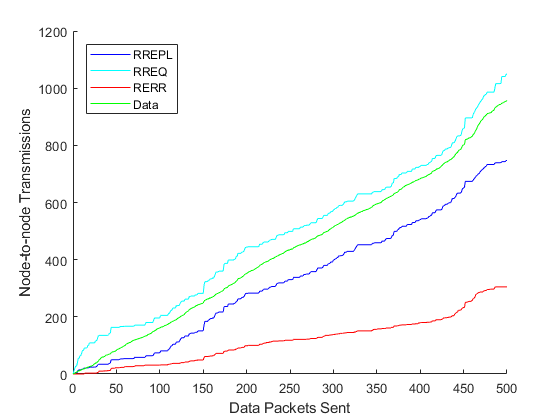
\includegraphics[width=3in]{movement_10.png}
	\caption{Network overhead with nodes moving every 10 packets sent}
	\label{fig:movement_10}
\end{figure}

Figure \ref{fig:hops} shows the number of hops required for each transmission. Although the numbers are not initially as dissimilar as might be expected, it is clear that the "movement every 10 packets" data set had consistently higher transmissions counts towards the upper end. The "no movement" data set also had a few towards the high end as well. This represents the initial flooding, which requires all nodes in the network to send messages. This flooding is required, to some degree, at all levels and is what evens out the hop count statistics here.

\begin{figure}[ht]
	\centering
	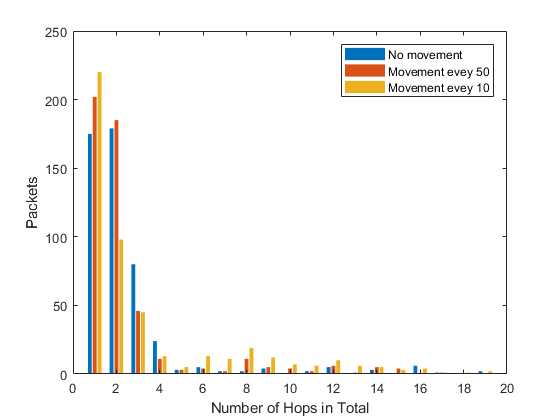
\includegraphics[width=3in]{hops_overall.png}
	\caption{Number of hops for various types of motion}
	\label{fig:hops}
\end{figure}

\section{Future Work}

Although this simulation provides an excellent base-level teaching tool, it falls short of accurate analysis in several areas. The foremost improvement that could be made would be to implement node queuing. While this would require a large burden of additional work, it would garner some interesting insights into node mechanics and provide a more realistic reflection of how ad-hoc networks truly perform. 

Additionally, to enhance the usefulness of this tool, it would be beneficial to be able to compare AODV to another routing protocol like destination-sequenced distance-vector (DSDV)  or dynamic source routing (DSR). Being able to compare and contrast the differences and weight the benefits of AODV would be a valuable opportunity.

\section{Conclusions}

The MATLAB-based ad-hoc on-demand distance vector (AODV) simulation presented above provides a meaningful method of demonstrating basic routing concepts quickly and easily, circumventing the learning curve of more specialized network simulation tools and facilitation visual learning. The MATLAB environment provides for easy inspection and expansion into additional analysis function. The examples and analysis presented serve as sufficient proof-of-concept of this endeavor to emulate AODV.

\section{lorem}
\lipsum

\bibliographystyle{IEEEtran}
\bibliography{sources}

\end{document}



